\documentclass{article}%
\usepackage[T1]{fontenc}%
\usepackage[utf8x]{inputenc}%
\usepackage{lmodern}%
\usepackage{textcomp}%
\usepackage{lastpage}%
\usepackage{ascii}%
\usepackage{graphicx}%
\usepackage{fancyhdr}%
%
\fancypagestyle{header}{ 
\renewcommand{\headrulewidth}{0pt}%
\renewcommand{\footrulewidth}{0pt}%
\fancyhead{ 
}%
\fancyfoot{ 
}%
\fancyhead[C]{ 
CHAPTER ONE
}%
\fancyfoot[C]{ 
}
}%
%
\begin{document}%
\normalsize%


\begin{figure}[h!]%
\centering%
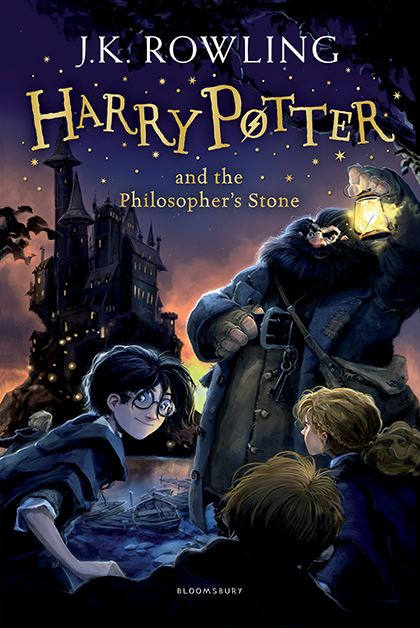
\includegraphics[width=300px]{C:/Users/sastr/Documents/ComputerScience/FinalProject/{./static/img/harryPotter}.jpg}%
\end{figure}

%
\newpage%
\asciifamily%
\centering%
\begin{Huge}%
\textbf{HARRY POTTER \newline%
}%
\end{Huge}%
\begin{Large}%
\textbf{And the Philosopher's Stone}%
\end{Large}%
\newpage%
\section*{ALSO BY J.K ROWLING}%
\label{sec:ALSO BY J.K ROWLING}%
\subsection*{Harry Potter and the Sorcerers Stone}%
\label{subsec:Harry Potter and the Sorcerers Stone}%
Year One at Hogwarts

%
\subsection*{Harry Potter and the Chamber of Secrets}%
\label{subsec:Harry Potter and the Chamber of Secrets}%
Year Two at Hogwarts

%
\subsection*{Harry Potter and the Prisoner of Azkaban}%
\label{subsec:Harry Potter and the Prisoner of Azkaban}%
Year Three at Hogwarts

%
\subsection*{Harry Potter and the Goblet of Fire}%
\label{subsec:Harry Potter and the Goblet of Fire}%
Year Four at Hogwarts

%
\subsection*{Harry Potter and the Oder of the Phoenix}%
\label{subsec:Harry Potter and the Oder of the Phoenix}%
Year Five at Hogwarts

%
\subsection*{Harry Potter and the Half{-}Blood Prince}%
\label{subsec:Harry Potter and the Half{-}Blood Prince}%
Year Six at Hogwarts

%
\subsection*{Harry Potter and the Deathly Hallows}%
\label{subsec:Harry Potter and the Deathly Hallows}%
Year Seven at Hogwarts

%
\newpage%
\begin{Large}%
\textbf{For Sean D. F Harris \newline%
 \newline%
}%
\end{Large}%
\begin{Large}%
\textbf{Getaway Driver and Foul{-}Weather Friend \newline%
}%
\end{Large}%
\begin{small}%
Text copywrite @ 1999 by J.K Rowling.\newline%
	Donec pellentesque libero id tempor aliquam. Maecenas a diam at metus varius\newline%
			rutrum vel in nisl. Maecenas a est lorem. Vivamus tristique nec eros ac\newline%
			hendrerit. Vivamus imperdiet justo id lobortis luctus. Sed facilisis ipsum ut\newline%
			tellus pellentesque tincidunt. Mauris libero lectus, maximus at mattis ut,\newline%
			venenatis eget diam. Fusce in leo at erat varius laoreet. Mauris non ipsum\newline%
			pretium, convallis purus vel, pulvinar leo. Aliquam lacinia lorem dapibus\newline%
			tortor imperdiet, quis consequat diam mollis.%
\end{small}%
\newpage%
\centering%
\section*{CONTENTS Numbering}%
\label{sec:CONTENTS Numbering}%
\begin{description}%
\centering%
\item[ONE]%
The first item%
\item[TWO]%
The second item%
\item[THREE]%
The third etc \ldots%
\end{description}

%
\centering%
\section*{CONTENTS Sections}%
\label{sec:CONTENTS Sections}%
\subsection*{ONE}%
\label{subsec:ONE}%
The first item

%
\subsection*{TWO}%
\label{subsec:TWO}%
The second item

%
\subsection*{THREE}%
\label{subsec:THREE}%
The third etc \textbackslash{}ldots

%
\newpage%
\pagestyle{header}%


\begin{figure}[h!]%
\centering%
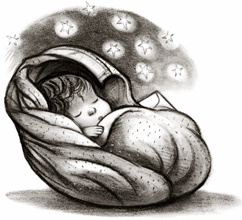
\includegraphics[width=200px]{C:/Users/sastr/Documents/ComputerScience/FinalProject/{./static/img/baby}.jpg}%
\end{figure}

%
\section*{THE BOY WHO LIVED}%
\label{sec:THE BOY WHO LIVED}%
\flushleft%
 Not for the first time, an argument had broken out over breakfast at number four, Privet Drive.\newline%
	Mr. Vernon Dursley had been woken in the early hours of the morning by a loud, hooting noise from his nephew\newline%
	Harry’s room.“Third time this week!” he roared across the table. “If you can’t control that owl, it’ll have to go!” \newline%
	Harry tried, yet again, to explain.“She’s bored,” he said. “She’s used to flying around outside.\newline%
	If I could just let her out at night —” “Do I look stupid?” snarled Uncle Vernon, a bit of fried egg dangling\newline%
	from his bushy mustache. “I know what’ll happen if that owl’s let out.” He exchanged dark looks with his wife, Petunia. \newline%
	Harry tried to argue back but his words were drowned by a long, loud belch from the Dursleys’ son, Dudley.\newline%
	“I want more bacon.” “There’s more in the frying pan, sweetums,” said Aunt Petunia,\newline%
	turning misty eyes on her massive son. “We must build you up while we’ve got the chance. . . .\newline%
	I don’t like the sound of that school food. . . .” “Nonsense, Petunia, I never went hungry when I was at Smeltings,”\newline%
	said Uncle Vernon heartily. “Dudley gets enough, don’t you, son?” \newline%
\newline%
	Dudley, who was so large his bottom drooped over either side of the kitchen chair, grinned and turned to Harry.\newline%
	“Pass the frying pan.” “You’ve forgotten the magic word,” said Harry irritably.\newline%
	The effect of this simple sentence on the rest of the family was incredible: Dudley gasped and fell off his chair\newline%
	with a crash that shook the whole kitchen; Mrs. Dursley gave a small scream and clapped her hands to her mouth;\newline%
	Mr. Dursley jumped to his feet, veins throbbing in his temples. “I meant ‘please’!” said Harry quickly.\newline%
	“I didn’t mean —” “WHAT HAVE I TOLD YOU,” thundered his uncle, spraying spit over the table,\newline%
	“ABOUT SAYING THE ‘M’ WORD IN OUR HOUSE?” “But I —” “HOW DARE YOU THREATEN DUDLEY!” roared Uncle Vernon,\newline%
	pounding the table with his fist. “I just —” “I WARNED YOU! I WILL NOT TOLERATE MENTION OF YOUR ABNORMALITY\newline%
	UNDER THIS ROOF!” Harry stared from his purple{-}faced uncle to his pale \newline%
	aunt, who was trying to heave Dudley to his feet. \newline%
\newline%
	Dudley hitched up his trousers, which were slipping down his fat bottom. “Why’re you staring at the hedge?” \newline%
	he said suspiciously. “I’m trying to decide what would be the best spell to set it on fire,” said Harry.\newline%
	Dudley stumbled backward at once, a look of panic on his fat face. “You c{-}can’t — Dad told you you’re\newline%
	not to do m{-}magic — he said he’ll chuck you out of the house — and you haven’t got anywhere else to \newline%
	go — you haven’t got any friends to take you —” “Jiggery pokery!” said Harry in a fierce voice. \newline%
	“Hocus pocus — squiggly wiggly —” “MUUUUUUM!” howled Dudley, tripping over his feet as he dashed\newline%
	back toward the house. “MUUUUM! He’s doing you know what!” Harry paid dearly for his moment of fun.\newline%
	As neither Dudley nor the hedge was in any way hurt, Aunt Petunia knew he hadn’t really done magic,\newline%
	but he still had to duck as she aimed a heavy blow at his head with the soapy frying pan.\newline%
	Then she gave him work to do, with the promise he wouldn’t eat again until he’d finished.\newline%
	While Dudley lolled around watching and eating ice cream, Harry cleaned the windows,\newline%
	washed the car, mowed the lawn, trimmed the flowerbeds, pruned and watered the roses, \newline%
	and repainted the garden bench. The sun blazed overhead, burning the back of his neck. \newline%
	Harry knew he shouldn’t have risen to Dudley’s bait, but Dudley had said the very thing\newline%
	Harry had been thinking himself . . . maybe he didn’t have any friends at Hogwarts. . . . \newline%
	Wish they could see famous Harry Potter now, he thought savagely as he spread manure on the flower beds,\newline%
	his back aching, sweat running down his face. It was half past seven in the evening when at last, exhausted,\newline%
	he heard Aunt Petunia calling him. “Get in here! And walk on the newspaper!” Harry moved gladly\newline%
	into the shade of the gleaming kitchen. On top of the fridge stood tonight’s pudding: a huge mound of \newline%
	whipped cream and sugared violets. A loin of roast pork was sizzling in the oven. “Eat quickly!\newline%
	The Masons will be here soon!” snapped Aunt Petunia, pointing to two slices of bread and a lump\newline%
	of cheese on the kitchen table. She was already wearing a salmon{-}pink cocktail dress. Harry \newline%
	washed his hands and bolted down his pitiful supper. The moment he had finished, Aunt Petunia\newline%
	whisked away his plate. “Upstairs! Hurry!” \newline%
\newline%
	As he passed the door to the living room, Harry caught a glimpse of Uncle Vernon and Dudley in bow ties\newline%
	and dinner jackets. He had only just reached the upstairs landing when the doorbell rang and \newline%
	Uncle Vernon’s furious face appeared at the foot of the stairs. “Remember, boy — one sound —” \newline%
	Harry crossed to his bedroom on tiptoe, slipped inside, closed the door, and turned to collapse on his bed.\newline%
	The trouble was, there was already someone sitting on it.

%
\end{document}